\DiaryEntry{Distance between (Random) Points on Lines, II}{2017-11-14}{Stochastic}

This entry is an extension to \ref{2016-07-11:entry}; basically a generalization of the results presented there.

\subsection{Expected Distance between two random Points on two parallel Lines}

We have a two parallel lines, each of length $B$ and spaced apart from each other by $L$. The problem geometry is shown below

\begin{figure}[H]
	\centering
	
\includegraphics[scale=0.7]{images/expected_distances_02_01.png}
\end{figure}

The squared distance is given by this expression:

\bee
d(x_1, x_2) = (x_2 - x_1)^2 + L^2
\eee

The expected value of the squared distance is then

\bee
\mE(d^2) = \int_{x_1=0}^B \int_{x_2=0}^B d^2(x_1, x_2) f(x_1) f(x_2) dx_1 dx_2
\eee

with $f(x_1), f(x_2)$ denoting the pdf of the x variables $x_1$ and $x_2$, respectively. These are assumed to be uniform; i.e. $f(x_1)=f(x_2)=1/B$ and the expectation therefore becomes

\bee
\mE(d^2) = \frac{1}{B^2} \int_{x_1=0}^B \int_{x_2=0}^B (x_2 - x_1)^2 + L^2 dx_1 dx_2 = \cdots = \frac{B^2}{6} + L^2
\eee

We can simulate this for different values of $L$ and $B$ in Julia \\
(\verb| JuliaStuff/stochastic/dist_in_line.jl|) 
and check that the simulation results match the analytical results.

In a similar spirit, we can formulate the expected value of the distance,

\bee
\mE(d) = \frac{1}{B^2} \int_{x_1=0}^B \int_{x_2=0}^B \sqrt{(x_2 - x_1)^2 + L^2} dx_1 dx_2,
\eee

however getting a closed form expression seems to be impossible. We can use \verb|maxima| to solve the integrals for e.g. $L=2, B=1$ and obtain 

\bee
\mE(d) = \frac{12 \operatorname{asinh}\left( \frac{1}{2}\right) -7 \sqrt{5}+16}{3} \approx 2.040688686072238
\eee

and for $L=1, B=1$ we get $\mE(d) \approx 1.076635732895178$. Both of these values match closely with the simulated results.

\subsection{Expected Distance between two random Points on two perpendicular Lines}

Let us try another problem geometry and show that we can have fun with this one as well.

\begin{figure}[H]
	\centering
	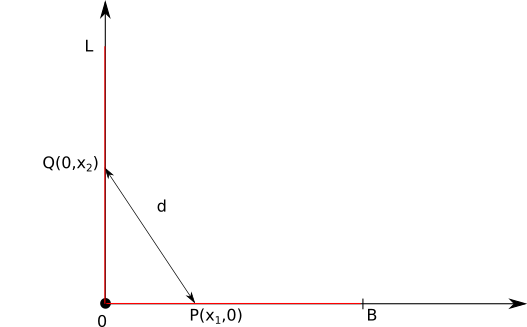
\includegraphics[scale=0.7]{images/expected_distances_02_02.png}
\end{figure}

Here the squared distance is given by

\bee
d^2(x_1, x_2) = x_1^2 + x_2^2
\eee

and assuming uniform distribution of the points $P$ and $Q$ in the interval $[0,L)$, we have

\bee
\mE(d^2) = \frac{1}{L^2} \int_{x_1=0}^B \int_{x_2=0}^B x_1^2 + x_2^2 dx_1 dx_2 = \cdots = \frac{2B^2}{3}
\eee

The expected value of the distance, $\mE(d)$ can be obtained in a simialr fashion, although the integration cannot be done in closed form

\bee
\mE(d) = \frac{1}{L^2} \int_{x_1=0}^B \int_{x_2=0}^B \sqrt{x_1^2 + x_2^2} dx_1 dx_2
\eee

Comparison of simulation and analytical results show that they match closely.